%! Author = joels
%! Date = 07/01/2022

%Sie können ...
%• Definition und Grundprinzipien eines Services (Dienstes) formulieren.
%• Service-Lifecycle aufzeigen.
%• das fundamentale SOA-Dreieck aufzeichnen.
%• Services mit SoaML modellieren.
%• synchrone Web Services wie SOAP/REST darlegen.
%• asynchrone Kommunikation mittels MOM ausführen.
%• den Aufbau der elektronischen Nachricht erläutern.
%• die Schritte der API Entwicklung erklären.
%• die Funktionen des API Managements nennen.
%• API Security mit SAML bzw. OAuth 2.0 einordnen.

\section{Service Oriented Architecture}
\subsection{Synchrone Web Services}
\begin{itemize}[topsep=0pt, leftmargin=3mm]
    \setlength\itemsep{-0.3em}
    \item Zustandsbehaftet
    \SubItem SOAP - Simple Object Access Protocol
    \item Zustandslos
    \SubItem REST
    \SubItem OData
    \SubItem GraphQL
    \SubItem gRPC
\end{itemize}
\subsection{Protokolle}
\textbf{E-Mail:}
\begin{itemize}[topsep=0pt, leftmargin=3mm]
    \setlength\itemsep{-0.3em}
    \item SMTP (Versenden)
    \item POP (Empfangen)
    \item IMAP (synchronisieren von Mails)
\end{itemize}
\textbf{Message Oriented Middleware (MOM, Message Broker):}
\begin{itemize}[topsep=0pt, leftmargin=3mm]
    \setlength\itemsep{-0.3em}
    \item Für asynchrone Kommunikation.. z.B. RabbitMQ
    \item AMQP
    \item JMS
    \item MQTT (IoT)
\end{itemize}
\subsection{Netzwerk-Sicherheitsarchitektur:}
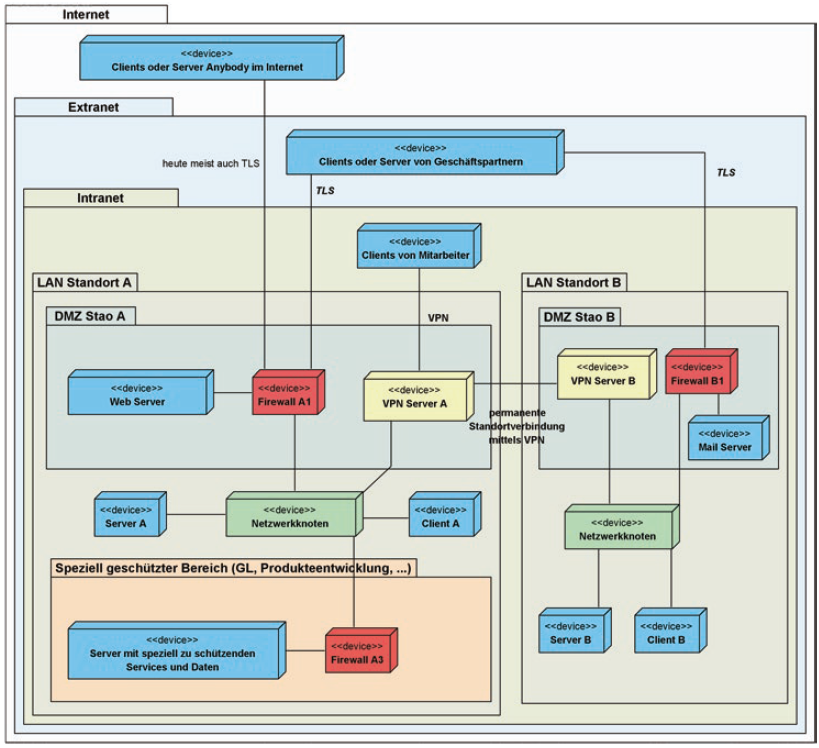
\includegraphics[width=\linewidth]{netzwerksicherheit_architektur}
\subsection{API-Gateway}
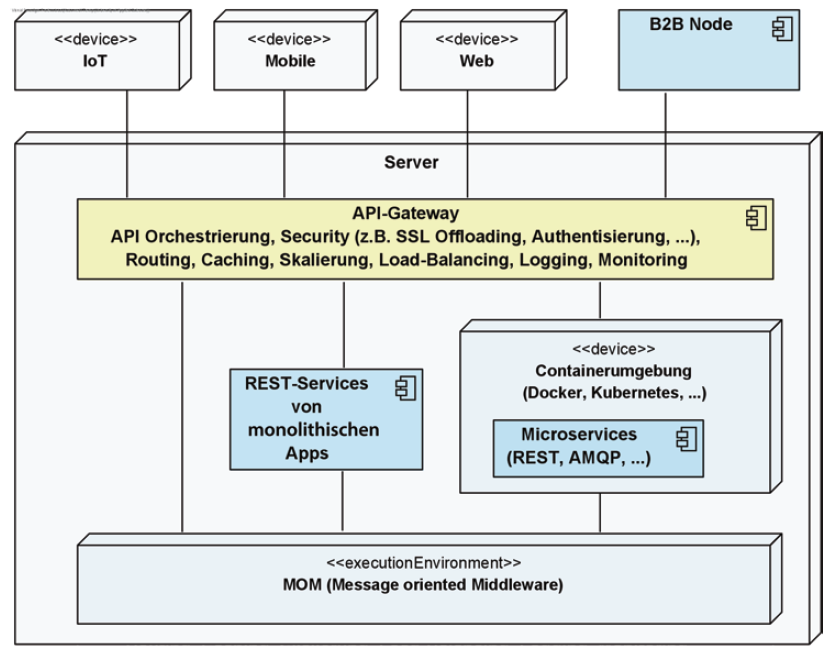
\includegraphics[width=\linewidth]{api_gateway}